土耳其的盐湖盆地对于保护生物多样性非常重要,根据国际标准被归类为湿地。它也是土耳其保有鸟类最多的湖泊之一。有鸟类85种,昆虫129种(其中4种是特有的),15种哺乳动物和38种特有的植物。该湖满足了土耳其约40\%的食盐需求(作为食用盐)。盐湖中的盐是由气象水排入地下并融化先前形成的盐穹顶,并沿构造线携带它们而形成的。盐湖中的盐生产是通过在阳光下蒸发湖水来完成的。我们利用太阳能通过池式系统制盐。

\begin{figure}[h]
	\centering
	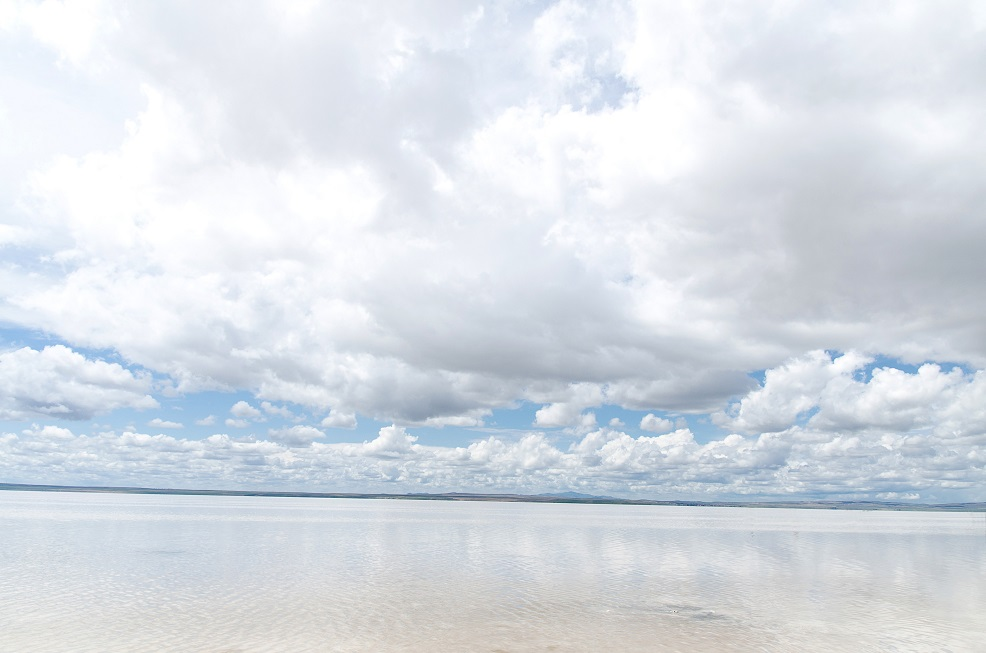
\includegraphics[width=10cm]{./pic/t15-1.jpg}
	\caption*{盐湖}
\end{figure}

食用盐是最常见的家用化学品之一。它是97\%到99\%的氯化钠,它是化学式为NaCl的离子化合物,代表钠和氯离子的比例为1:1。NaCl是最影响海水和许多多细胞生物体细胞外液盐度的化合物。食用盐的可食用形式通常用作调味品和食品防腐剂。钠的第二个主要应用是在亚冰冻天气中,用氯化物给道路除冰。大量氯化钠还用于许多工业过程中,例如氯碱工业和纯碱工业以及其他工业用途:水软化,医药,农业,消防和清洁剂。NaCl直接或间接用于生产许多钠化合物。世界上大部分产量都为钠化合物。下图显示了从NaCl制备一些钠化合物的方法。

\begin{figure}[h]
	\centering
	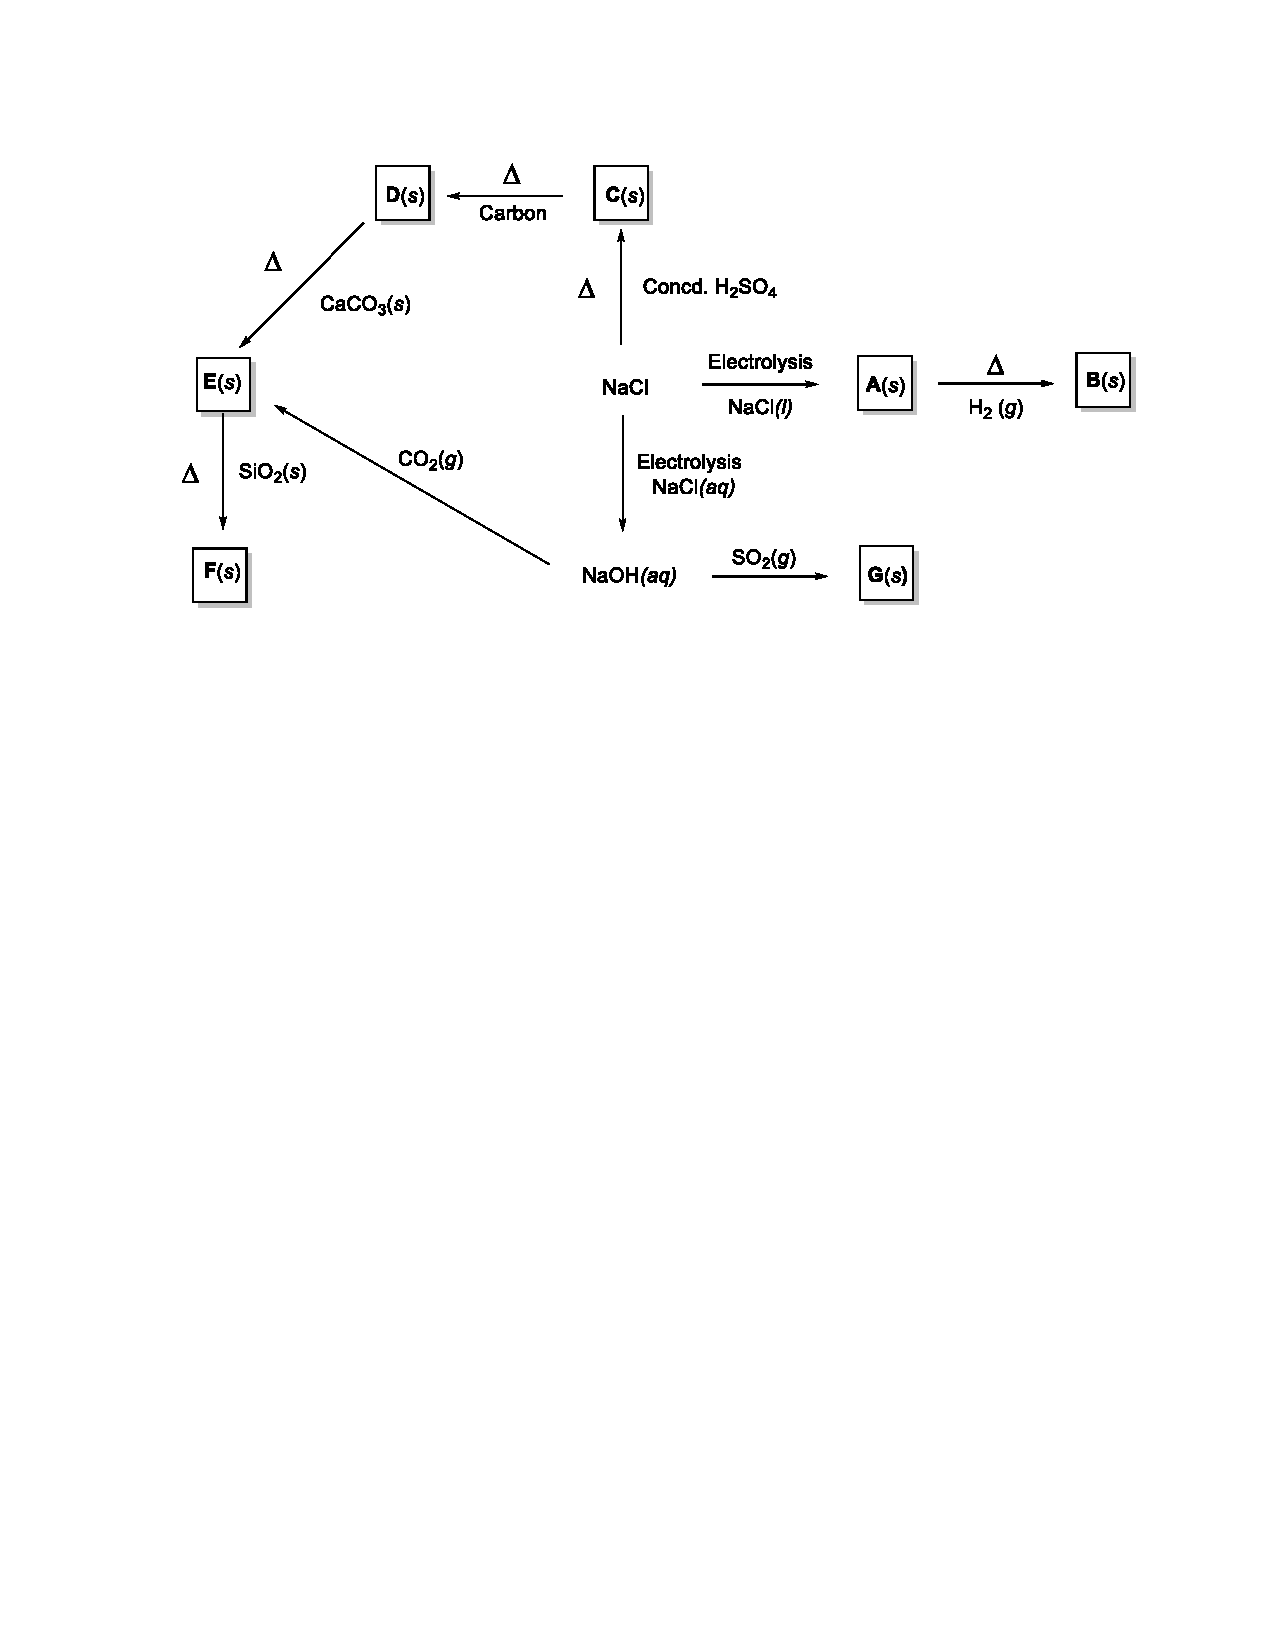
\includegraphics[width=14cm]{./pic/t15-2.pdf}
	\caption*{从NaCl开始制备一些钠化合物。}
\end{figure}

\noindent\textbf{15.1.} 写出\textbf{A}-\textbf{G}的分子式

碳酸钠(Na\textsubscript{2}CO\textsubscript{3},苏打粉),主要用于制造玻璃。它主要来源于天然产物,例如天然碱,Na\textsubscript{2}CO\textsubscript{3}·NaHCO\textsubscript{3}·$n$H\textsubscript{2}O。其主要可通过NaCl,CaCO\textsubscript{3},NH\textsubscript{3}用一个比利时化学家Ernest Solvay在1863年发明的方法生产。关键步骤包括NH\textsubscript{3}(g)和CO\textsubscript{2}(g)在饱和NaCl(aq)中反应。在所有可能从混合物结晶的离子型化合物中(NaCl,NH\textsubscript{4}Cl,NaHCO\textsubscript{3},NH\textsubscript{4}HCO\textsubscript{3}),溶解度最小的是碳酸氢钠(NaHCO\textsubscript{3})。它通过过滤分离出来,然后通过加热转化为碳酸钠(Na\textsubscript{2}CO\textsubscript{3})。根据解释,

\noindent\textbf{15.2.} 配平下面的方程式

$\ce{NaCl(aq) + CO2(g) + NH3(g) + H2O ->}$

$\ce{2NaHCO3(s) ->[\Delta]}$

\noindent\textbf{15.3.}
使用CaCO\textsubscript{3}(石灰石),你怎样才能获得你想要的CO\textsubscript{2}气体来生产NaHCO\textsubscript{3}?

\noindent\textbf{15.4.}
写出CaCO\textsubscript{3}的包含所有共振式的Lewis结构,并标出每个原子的形式电荷。

\noindent\textbf{15.5.}
描述CO$_3^{2-}$的分子几何结构并提出中心原子合理的杂化方式。

\noindent\textbf{15.6.}
按照键长增长的顺序排列CO$_3^{2-}$,CO,CO\textsubscript{2}

NaCl结晶为面心立方(fcc)结构。NaCl的密度为2180
kg m\textsuperscript{−3},Na\textsuperscript{+}的离子半径为99pm。

\noindent\textbf{15.7.} 在晶胞中有多少原子?什么原子占据八面体空隙?

\noindent\textbf{15.8.}
计算NaCl的晶胞长度和Cl\textsuperscript{−}的离子半径(用pm)

碱金属与氧气快速反应,生成几种不同的离子型氧化物。在适当的条件下,通常通过仔细控制氧气,每种碱金属都能生成氧化物M\textsubscript{2}O。
锂与过量氧气反应生成\textbf{A}和少量的\textbf{B}。钠与过量的氧气反应生成大部分\textbf{C}和少量\textbf{D}。钾,铷和铯反应与过量的氧气形成\textbf{E},\textbf{F}和\textbf{G}。

\noindent\textbf{15.9.} \textbf{A}-\textbf{G}是哪些常见的金属氧化物?

\noindent\textbf{15.11.} 画出过氧和超氧离子的分子轨道能级图并比较它们的键长和能量。

当LiClO\textsubscript{4},NaClO\textsubscript{4}和KClO\textsubscript{4}从水溶液结晶时,它们可能包含或不包含称为结晶水的水分子作为固体结构的一部分,尽管没有简单的规则可以确定地预测离子在固态中是否保留其全部或部分水化球,具有高电荷密度的阳离子倾向于将其全部或部分水化球保留在固态中。当阳离子具有低电荷密度时,它们往往会失去其水合球;因此,它们倾向于形成无水盐。Li\textsuperscript{+},Na\textsuperscript{+}和K\textsuperscript{+}的离子半径分别为76 pm,102 pm和138 pm。

\noindent\textbf{15.12.} 计算这些离子的电荷密度(单位用C mm\textsuperscript{−3})

\noindent\textbf{15.13.} 哪种高氯酸盐最易形成无水化合物?
